\chapter{Other methods and optimizations}\label{otherMethods}

In the previous chapters two methods to estimate the location of a flare have been presented. 

Here, other possible optimizations are considered that could be used to, in the future, extend the algorithm and perhaps improve its performance and accuracy.

While some are completely different methods, others are optimizations that can be built on top of any approach.

\section{Hill Climbing}

Using the decrease range method in chapter 6 we could see the plot of all the possibilities the algorithm considers:

\begin{figure}[!htb]
	\begin{centering}
		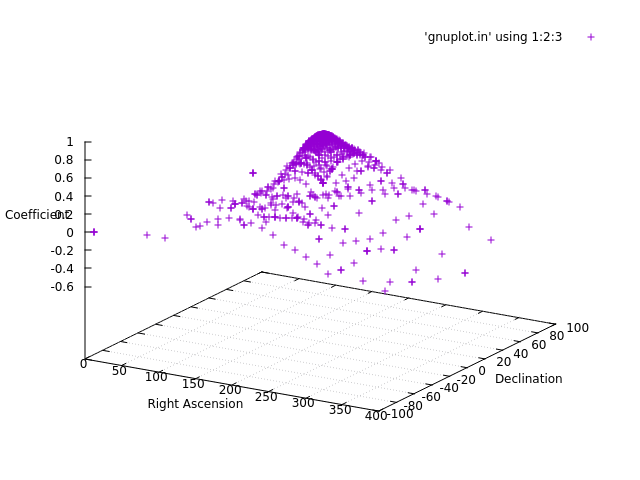
\includegraphics[width=0.5\linewidth]{images/ch6/hillClimbing/resultsAll.png}
		\caption{All visited candidates of the solution space}
		\label{fig:solutionSpace}
	\end{centering}
\end{figure}

In this solution space, there appears to be a "hill" (our solution) so an attempt to solve the problem using a \textit{Hill Climbing} approach was also considered.

Hill Climbing is an heuristic search algorithm that moves through the solution space of a problem by finding the best neighbour of the current solution until it can not progress any more. Seeing the previous figure we thought it could be interesting to test this method for our problem, so a simple greedy algorithm was implemented as a first attempt to test if the method could work.

The following is the implementation of such test, which checks its surrounding neighbours and moves to the best one (the objective function is the correlation) until the solution can not be improved any further.

\begin{minipage}{\linewidth}
	\begin{lstlisting}[language=c, caption=Hill Climbing]
	// Starting position
	sourceInfo current;
	current.ra = 160;
	current.dec = -20;
	int i = 0;
	// Loop with limit or until no progress can't be made
	while (++i < 100) {
		vector<sourceInfo> candidates = getNeighbourList(current);
		sourceInfo newCandidate = getBestCandidate(candidates);
		if (newCandidate < current) {
			break;
		}
		current = newCandidate;
	}
	\end{lstlisting}
\end{minipage}

The following figure shows the results of the execution for two different starting states. For both of them, the algorithm ran until it could not progress any further (wasn not interrupted by the iteration limit). The plots contain both the possibilities considered by the decrease range method (in purple, the same plot as \ref{fig:solutionSpace}), and the path taken by the greedy algorithm (in green).

\begin{figure}[!htb]
	\begin{subfigure}[b]{0.5\textwidth}
		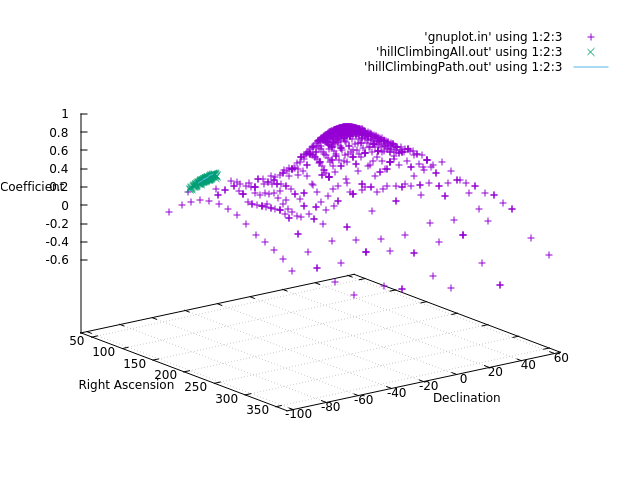
\includegraphics[width=\linewidth]{images/ch6/hillClimbing/resultsPathBad.png}
		\caption{Start: ra=100$^{\circ}$, dec=-60$^{\circ}$}
	\end{subfigure}
	\hfill
	\begin{subfigure}[b]{0.5\textwidth}
		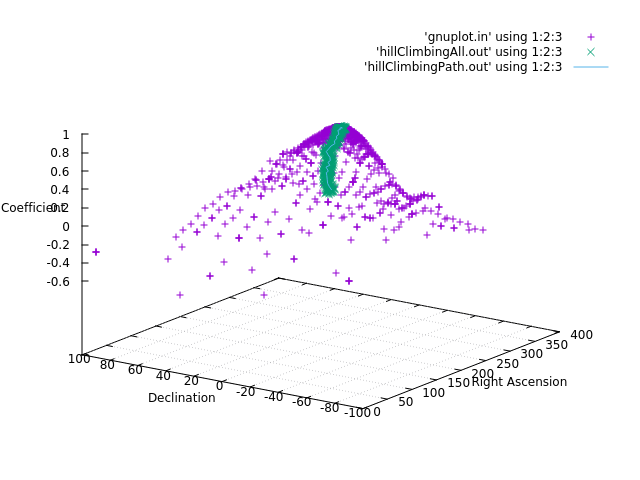
\includegraphics[width=\linewidth]{images/ch6/hillClimbing/resultsPathGood.png}
		\caption{Start: ra=160$^{\circ}$, dec=-20$^{\circ}$}
	\end{subfigure}
	\caption{Paths taken by the Hill Climbing algorithm}
	\label{fig:hillClimbingPaths}
\end{figure}

Visually, we can see that the number of considered possibilities is inferior and the top is reached for case (b), but a problem appears: \textbf{a local maxima}.

If we take a starting right ascension of 160$^{\circ}$ and a declination of -20$^{\circ}$, the algorithm takes a path that gets to the top of our solution, yielding similar results to the previous, decrease range method.

However, with a starting right ascension of 100$^{\circ}$ and a declination of -60$^{\circ}$, the algorithm finds a local maxima on its way and cannot progress to the real best solution.

As a result, the Hill Climbing approach is not reliable for all cases, considering that local maxima may exist for our type of problem, leading to incorrect estimations in some cases.

\section{Simulated Annealing}

Simulated Annealing is an heuristic search algorithm that approximates the optimal solution of a problem, similar to Hill Climbing. The main difference is the use of probability to accept a solution as better than the current one, to be able to explore other areas of the solution space.

A possible solution to the problem of local maxima seen in the previous section would be using the Simulated Annealing algorithm so that other parts of the solution space could be explored, finding other paths that might lead to our desired solution, instead of only focusing on one path that could get stuck in a local maxima.

Although it might yield better results, simulated annealing approximates the optimal solution, but does not guarantee finding the global maxima.

\section{OpenMP}

OpenMP (Open Multi-Processing) is an specification for compiler directives and library routines available for C, C++ and Fortran used for parallel programming.

Using OpenMP would not be an entirely different method, but rather an optimization that could be used with all the presented methods to try to parallelize some regions of the code. It would be feasible for our case considering it is available for both C++ and Fortran, the main languages used for the algorithms.

An example of how multi-processing could be used for the algorithm would be parallelizating the computation of the correlation in the decrease range method: each thread could read a part of the input and compute the necessary variables used to compute the final value of the correlation. Because these variables are sums, each thread could handle a part of the input and finally we could compute the total sum using OpenMP's reduction clause (which sums the values from each thread at the end of the partial loop). \\

These two possibilities (using OpenMP and Simmulated Annealing) could be implemented in the future if more tests were done with the algorithm, but for now we decided to focus on the methods from previous chapters.